\documentclass[border=6pt]{standalone}
\usepackage{tikz}
\usetikzlibrary{arrows.meta,positioning,calc,shapes.geometric,fit,backgrounds,patterns,matrix,decorations.pathreplacing}
\begin{document}
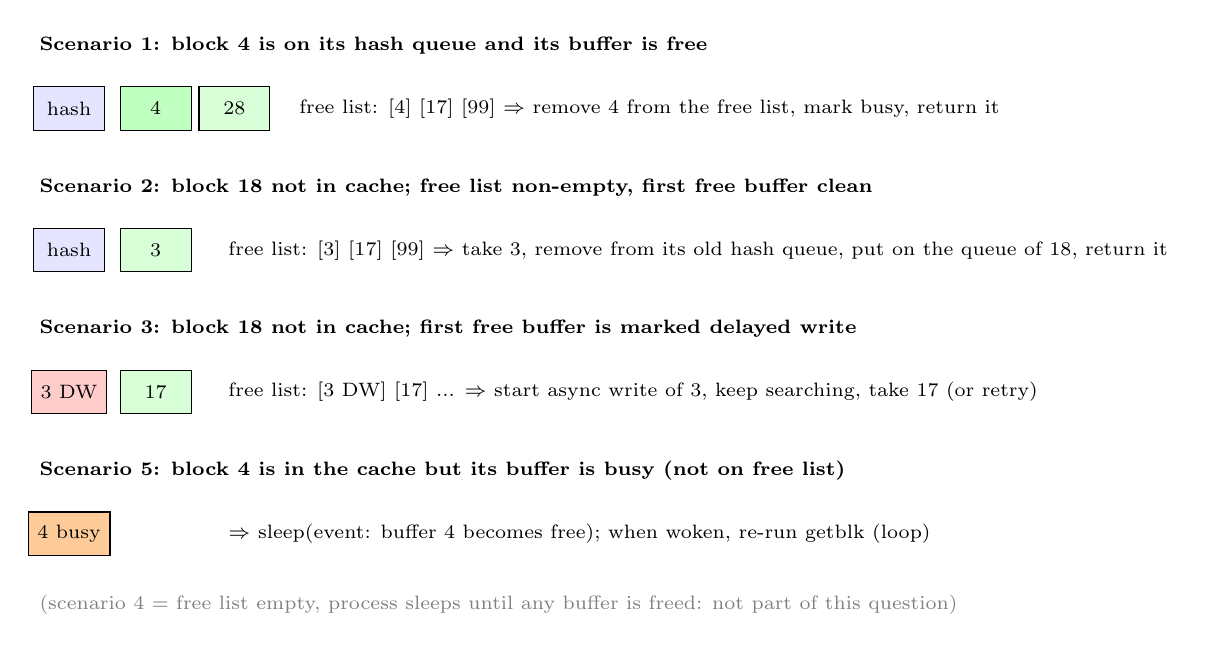
\begin{tikzpicture}[>=Stealth,font=\small]
\tikzstyle{b}=[draw,minimum width=0.9cm,minimum height=0.55cm,font=\scriptsize]
\tikzstyle{t}=[font=\scriptsize\bfseries,anchor=west]
% scenario 1
\node[t] at (0,0) {Scenario 1: block 4 is on its hash queue and its buffer is free};
\node[b,fill=blue!10] at (0.5,-0.8) {hash}; \node[b,fill=green!25] (a) at (1.6,-0.8) {4}; \node[b,fill=green!15] at (2.6,-0.8) {28};
\node[font=\scriptsize,anchor=west] at (3.3,-0.8) {free list: [4] [17] [99]  $\Rightarrow$ remove 4 from the free list, mark busy, return it};
% scenario 2
\node[t] at (0,-1.8) {Scenario 2: block 18 not in cache; free list non-empty, first free buffer clean};
\node[b,fill=blue!10] at (0.5,-2.6) {hash}; \node[b,fill=green!15] at (1.6,-2.6) {3};
\node[font=\scriptsize,anchor=west] at (2.4,-2.6) {free list: [3] [17] [99] $\Rightarrow$ take 3, remove from its old hash queue, put on the queue of 18, return it};
% scenario 3
\node[t] at (0,-3.6) {Scenario 3: block 18 not in cache; first free buffer is marked delayed write};
\node[b,fill=red!20] at (0.5,-4.4) {3 DW}; \node[b,fill=green!15] at (1.6,-4.4) {17};
\node[font=\scriptsize,anchor=west] at (2.4,-4.4) {free list: [3 DW] [17] ... $\Rightarrow$ start async write of 3, keep searching, take 17 (or retry)};
% scenario 5
\node[t] at (0,-5.4) {Scenario 5: block 4 is in the cache but its buffer is busy (not on free list)};
\node[b,fill=orange!40] at (0.5,-6.2) {4 busy};
\node[font=\scriptsize,anchor=west] at (2.4,-6.2) {$\Rightarrow$ sleep(event: buffer 4 becomes free); when woken, re-run getblk (loop)};
\node[font=\scriptsize,anchor=west,gray] at (0,-7.1) {(scenario 4 = free list empty, process sleeps until any buffer is freed: not part of this question)};
\end{tikzpicture}
\end{document}
